
%------------------------------------------------

\section{Acceptance-Rejection method}
\label{exer:acceptance_rejection}

\subsection{Hit-or-miss method}

\begin{enumerate}
	\item Generate $10^{6}$ points uniformly distributed with $x \in [-1, 1]$ and $y \in [-1, 1]$.
	\item Compute the fraction of points falling inside a circle of radius 1.
	\item Repeat for $\mathrm{dim} = \{ 2, 3, 4, \cdots, 15 \}$.
	\item Plot the fraction of accepted points as a function of the dimension.
	\item Assign an uncertainty to your estimate of accepted points.
	\item Compare the plot with the theoretical expectation.
\end{enumerate}

\subsection{Hints for the solution}

The theoretical expectation is the ratio between the volume of an n-dimensional sphere and $2^{n}$.

As an uncertainty, we can use the variance of the binomial distribution.

(Figure~\ref{fig:acceptance_rejection})

\begin{figure}
	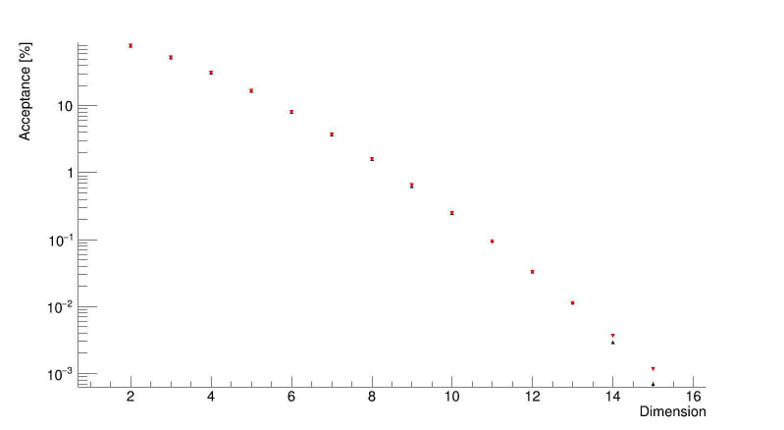
\includegraphics{exercise/acceptance_rejection_method.png}
	\caption[Acceptance as a function of the dimension.][6pt]{Acceptance as a function of the dimension for acceptance rejection method.}
	\label{fig:acceptance_rejection}
\end{figure}

($\hookleftarrow$ \ref{subsec:acceptance_rejection})
